\documentclass[journal,12pt,twocolumn]{IEEEtran}

\usepackage{setspace}
\usepackage{gensymb}
\singlespacing
\usepackage[cmex10]{amsmath}

\usepackage{amsthm}

\usepackage{mathrsfs}
\usepackage{txfonts}
\usepackage{stfloats}
\usepackage{bm}
\usepackage{cite}
\usepackage{cases}
\usepackage{subfig}

\usepackage{longtable}
\usepackage{multirow}

\usepackage{enumitem}
\usepackage{mathtools}
\usepackage{steinmetz}
\usepackage{tikz}
\usepackage{circuitikz}
\usepackage{verbatim}
\usepackage{tfrupee}
\usepackage[breaklinks=true]{hyperref}
\usepackage{graphicx}
\usepackage{tkz-euclide}

\usetikzlibrary{calc,math}
\usepackage{listings}
    \usepackage{color}                                            %%
    \usepackage{array}                                            %%
    \usepackage{longtable}                                        %%
    \usepackage{calc}                                             %%
    \usepackage{multirow}                                         %%
    \usepackage{hhline}                                           %%
    \usepackage{ifthen}                                           %%
    \usepackage{lscape}     
\usepackage{multicol}
\usepackage{chngcntr}

\DeclareMathOperator*{\Res}{Res}

\renewcommand\thesection{\arabic{section}}
\renewcommand\thesubsection{\thesection.\arabic{subsection}}
\renewcommand\thesubsubsection{\thesubsection.\arabic{subsubsection}}

\renewcommand\thesectiondis{\arabic{section}}
\renewcommand\thesubsectiondis{\thesectiondis.\arabic{subsection}}
\renewcommand\thesubsubsectiondis{\thesubsectiondis.\arabic{subsubsection}}


\hyphenation{op-tical net-works semi-conduc-tor}
\def\inputGnumericTable{}                                 %%

\lstset{
%language=C,
frame=single, 
breaklines=true,
columns=fullflexible
}
\begin{document}


\newtheorem{theorem}{Theorem}[section]
\newtheorem{problem}{Problem}
\newtheorem{proposition}{Proposition}[section]
\newtheorem{lemma}{Lemma}[section]
\newtheorem{corollary}[theorem]{Corollary}
\newtheorem{example}{Example}[section]
\newtheorem{definition}[problem]{Definition}

\newcommand{\BEQA}{\begin{eqnarray}}
        \newcommand{\EEQA}{\end{eqnarray}}
\newcommand{\define}{\stackrel{\triangle}{=}}
\bibliographystyle{IEEEtran}
\raggedbottom
\setlength{\parindent}{0pt}
\providecommand{\mbf}{\mathbf}
\providecommand{\pr}[1]{\ensuremath{\Pr\left(#1\right)}}
\providecommand{\qfunc}[1]{\ensuremath{Q\left(#1\right)}}
\providecommand{\sbrak}[1]{\ensuremath{{}\left[#1\right]}}
\providecommand{\lsbrak}[1]{\ensuremath{{}\left[#1\right.}}
\providecommand{\rsbrak}[1]{\ensuremath{{}\left.#1\right]}}
\providecommand{\brak}[1]{\ensuremath{\left(#1\right)}}
\providecommand{\lbrak}[1]{\ensuremath{\left(#1\right.}}
\providecommand{\rbrak}[1]{\ensuremath{\left.#1\right)}}
\providecommand{\cbrak}[1]{\ensuremath{\left\{#1\right\}}}
\providecommand{\lcbrak}[1]{\ensuremath{\left\{#1\right.}}
\providecommand{\rcbrak}[1]{\ensuremath{\left.#1\right\}}}
\theoremstyle{remark}
\newtheorem{rem}{Remark}
\newcommand{\sgn}{\mathop{\mathrm{sgn}}}
\providecommand{\abs}[1]{\left\vert#1\right\vert}
\providecommand{\res}[1]{\Res\displaylimits_{#1}}
\providecommand{\norm}[1]{\left\lVert#1\right\rVert}
%\providecommand{\norm}[1]{\lVert#1\rVert}
\providecommand{\mtx}[1]{\mathbf{#1}}
\providecommand{\mean}[1]{E\left[ #1 \right]}
\providecommand{\fourier}{\overset{\mathcal{F}}{ \rightleftharpoons}}
%\providecommand{\hilbert}{\overset{\mathcal{H}}{ \rightleftharpoons}}
\providecommand{\system}{\overset{\mathcal{H}}{ \longleftrightarrow}}
%\newcommand{\solution}[2]{\textbf{Solution:}{#1}}
\newcommand{\solution}{\noindent \textbf{Solution: }}
\newcommand{\cosec}{\,\text{cosec}\,}
\providecommand{\dec}[2]{\ensuremath{\overset{#1}{\underset{#2}{\gtrless}}}}
\newcommand{\myvec}[1]{\ensuremath{\begin{pmatrix}#1\end{pmatrix}}}
\newcommand{\mydet}[1]{\ensuremath{\begin{vmatrix}#1\end{vmatrix}}}
\numberwithin{equation}{subsection}
\makeatletter
\@addtoreset{figure}{problem}
\makeatother
\let\StandardTheFigure\thefigure
\let\vec\mathbf
\renewcommand{\thefigure}{\theproblem}
\def\putbox#1#2#3{\makebox[0in][l]{\makebox[#1][l]{}\raisebox{\baselineskip}[0in][0in]{\raisebox{#2}[0in][0in]{#3}}}}
\def\rightbox#1{\makebox[0in][r]{#1}}
\def\centbox#1{\makebox[0in]{#1}}
\def\topbox#1{\raisebox{-\baselineskip}[0in][0in]{#1}}
\def\midbox#1{\raisebox{-0.5\baselineskip}[0in][0in]{#1}}
\vspace{3cm}
\title{Assignment 1}
\author{Venkata Tejaswini Anagani - EE18BTECH11047}
\maketitle
\newpage
\bigskip
\renewcommand{\thefigure}{\theenumi}
\renewcommand{\thetable}{\theenumi}
Download all the codes and figures from
\begin{lstlisting}
https://github.com/anaganitejaswini/C-and-DS/gate_assignment
\end{lstlisting}
\section{Problem}
A queue is implemented using a non-circular singly linked list. The queue has a head pointer and a tail pointer, as shown in the figure. Let \emph{n} denote the number of nodes in the queue. Let \emph{enqueue} be implemented by inserting a new node at the head, and \emph{dequeue} be implemented by deletion of a node from the tail.


\begin{figure}[!bth]
    \centering
    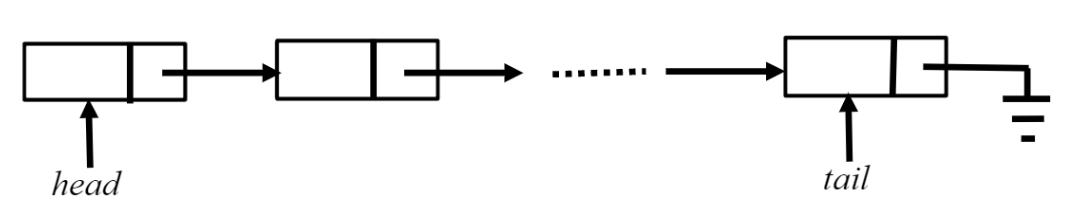
\includegraphics[scale=0.4]{figs/queue.png}
    \caption{}
    \label{fig1}
\end{figure}

What is the time complexity of the most time-efficient implementation of \emph{enqueue} and \emph{dequeue}, respectively, for this data structure?


\section{Solution}
\textbf{Enqueue:} The enqueue operation involves two operations:
\begin{itemize}
    \item Create a new node with the value to be inserted and point the next pointer of this node to the head of the linked list.
    \item Make the new node as the head of the linked list.
\end{itemize}
Creating a new node and changing two pointers can be performed in constant time. Therefore, time complexity of \emph{enqueue} operation is $\Theta (1)$ .
\\

\textbf{Dequeue: } The dequeue operation involves the following steps:
\begin{itemize}
    \item Delete the tail node.
    \item Traverse the linked list to find the address of the second last node and make the next pointer NULL. Update the tail pointer.
\end{itemize}

Since we are traversing the whole linked list, the time 
complexity of \emph{dequeue} operation is $\Theta (n)$ where n is the number of nodes in the linked list.
\\
\\
\textbf{Verification: } 


Below are the experimental plots of time complexities.

\begin{figure}[!ht]
    \begin{center}
    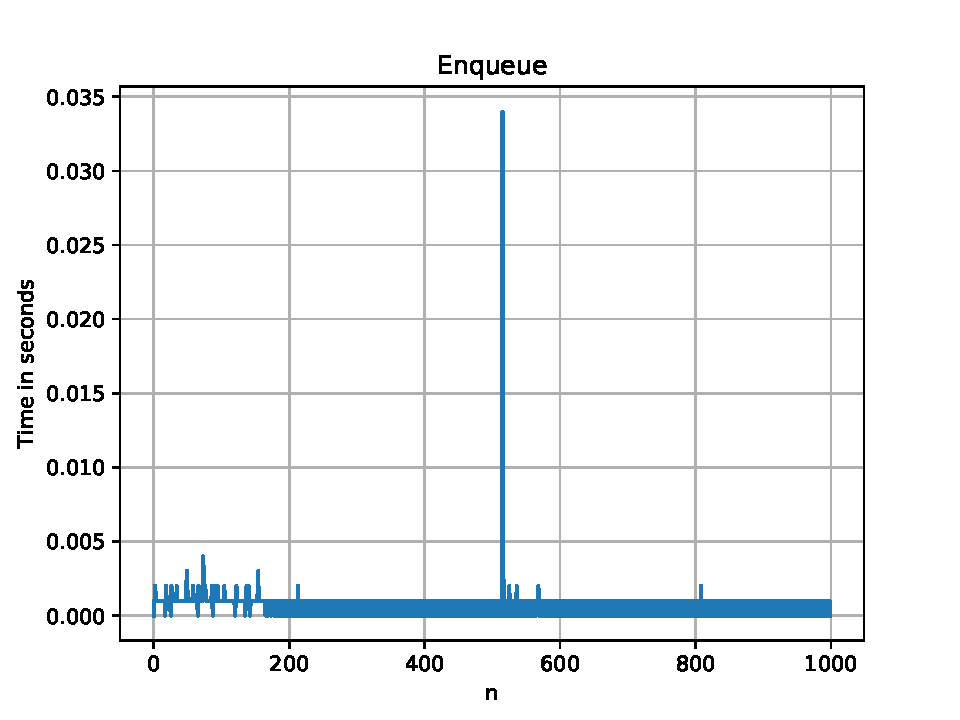
\includegraphics[width=\columnwidth]{./figs/enqueue}
    \end{center}
    \captionof{figure}{1}
    \label{fig2}	
\end{figure}


\begin{figure}[!ht]
    \begin{center}
    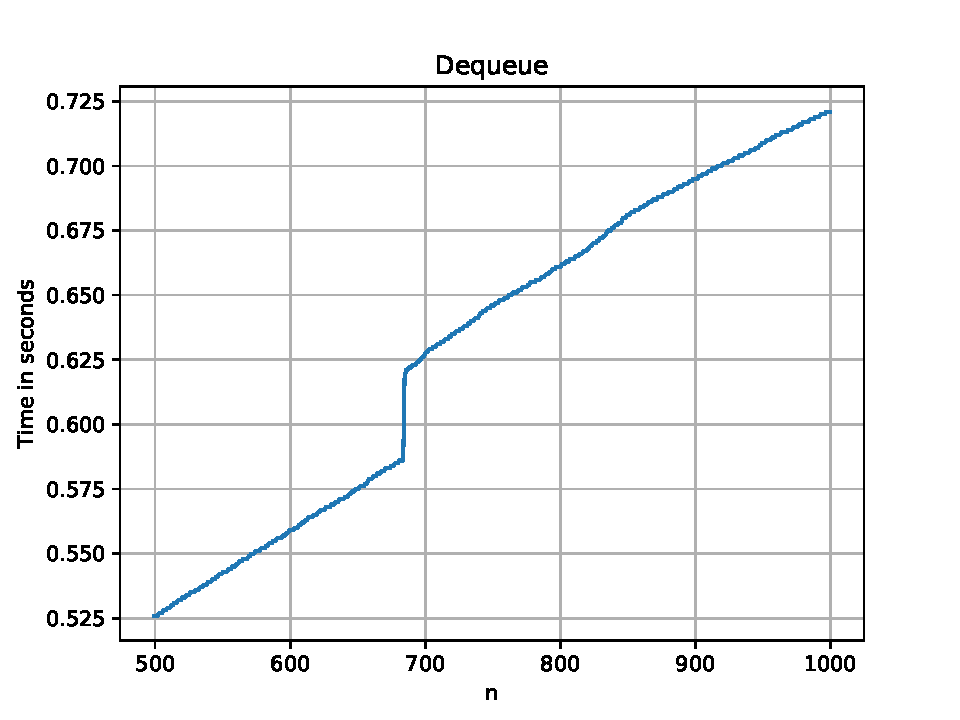
\includegraphics[width=\columnwidth]{./figs/dequeue}
    \end{center}
    \captionof{figure}{2}
    \label{fig3}	
\end{figure}

The following code executes enqueue and dequeue operations several times and stores the execution time values in a dat file.

\begin{lstlisting}
https://github.com/anaganitejaswini/C-and-DS/gate_assignment/codes/linked_list.c
\end{lstlisting}
The following python code plots the time complexity of enqueue and dequeue.
\begin{lstlisting}
https://github.com/anaganitejaswini/C-and-DS/gate_assignment/codes/time_complexity.py
\end{lstlisting}



Therefore, the time complexity of the most time efficient implementation of \emph{enqueue} and \emph{dequeue} respectively are $\Theta(1)$ and $\Theta(n)$.

\end{document}